\documentclass[a4paper,11pt]{article}
\usepackage{a4wide}
\usepackage{fullpage}
\usepackage[utf8x]{inputenc}
\usepackage[slovene]{babel}
\selectlanguage{slovene}
\usepackage[toc,page]{appendix}
\usepackage[pdftex]{graphicx} % za slike
\usepackage{setspace}
\usepackage{color}
\definecolor{light-gray}{gray}{0.95}
\definecolor{green}{RGB}{0,128,0}
\usepackage{listings} % za vključevanje kode
\usepackage{hyperref}
\renewcommand{\baselinestretch}{1.2} % za boljšo berljivost večji razmak
\renewcommand{\appendixpagename}{Priloge}

\lstset{ % nastavitve za izpis kode, sem lahko tudi kaj dodaš/spremeniš
language=c++,
basicstyle=\footnotesize,
basicstyle=\ttfamily\footnotesize\setstretch{1},
backgroundcolor=\color{light-gray},
}

\title{RIS - Poročilo}
\author{Jan Gulič, Luka Podgoršek, Rok Poje, Sašo Cvitkovič}
\date{\today}

\begin{document}

\maketitle
% ----------------------------- UVOD ---------------------------------------- %
\section{Uvod}

Pri predmetu Razvoj inteligentnih sistemov (RIS) smo ekipo z imenom \textbf{team theta} sestavljali:
\begin{itemize}
	\item Cvitkovič Sašo
	\item Gulič Jan
	\item Podgoršek Luka
	\item Poje Rok
\end{itemize}

% ----------------------------- OPIS PROBLEMA ---------------------------------------- %

\section{Opis problema}

Končna naloga je bila implementacija robotskega taksija. Poligon je predstavljal mesto, v katerem se je robot vozil in izpoljeval naloge. Mesto je bilo sestavljeno iz štirih ulic, štirih hiš in prometnih znakov, katere je robot moral upoštevati med samo vožnjo. Na začetku smo robota postavili v mesto in mu sporočili njegovo lokacijo. Nato je uporabnik preko telefona (uporabljena je bila Android aplikacija) sporočil robotu svoje ime in na kateri ulici se nahaja. Robot se je odpeljal na željeno ulico in poiskal uporabnika, ki ga je poklical. Nato je s potnikom opravil kratek dialog, preko katerega je izvedel željeno destinacijo. Uporabnika je odpeljal na destinacijo, kjer je moral poiskati stavbo. Stavbe so bile predstavljene kot barvni cilindri. Po uspešni dostavi se je robot odpeljal po naslednjega uporabnika. 
Robot je nalogo opravil, ko je uspešno odpeljal tri osebe na željeno destinacijo.\\


Slike mesta, obrazev in zgradb najdete v prilogi \ref{sec:slike}.

% ----------------------------- OPIS GLAVNIH NALOG ---------------------------------------- %

\subsection{Opis glavnih nalog -- REMOVE}
\subsubsection{Detekcija in razpoznava}
Robot je moral zaznati in razpoznati osebe, prometne znake in zgradbe.
\subsubsection{Dialog z osebo}
Robot je moral preko dialoga z osebo razpoznati ukaze in jih nato izvesti.
\subsubsection{Navigacija}
Robot se je moral znati navigirati v vnaprej pripravljeni mapi.

% ----------------------------- REALIZACIJA ZAHTEV ---------------------------------------- %

\section{Realizacija zahtev}
Zahteve, ki so obarvane z rdečo niso bile implementirane.

\begin{itemize}
	\color{green}
	\item Learn the appearance of nine faces
	\item {\color{red}Learn the appearance of five traffic signs}
	\item {\color{red}Learn the appearance of four buildings}
	\item Build the map of the competition area
	\item Manually mark the streets in the map
	\item Start at any position
	\item Travel around the city
	\item {\color{red}Detect and recognize the traffic signs}
	\item {\color{red}Follow the traffic rules}
	\item Detect and recognize the faces
	\item {\color{red}Detect and recognize the buildings}
	\item Wait and understand the dispatcher's commands
	\item Ask the individuals where to take them
	\item Take the person to the correct building
	\item {\color{red}Decide whether to take two persons together}
\end{itemize}

% ----------------------------- METODOLOGIJA ---------------------------------------- %

\section{Metodologija}
\subsection{Detekcija in razpoznava obrazev}

Detekcija obrazev: 
Razpoznava obrazev uporablja: haarcascade classifier

\subsection{Detekcija in razpoznava prometnih znakov}
\subsubsection{Upoštevanje prometnih znakov}
\subsection{Detekcija in razpoznava cilindrov}
\subsection{Navigacija}
\subsection{Dialog človek računalnik}

% ----------------------------- INTEGRACIJA ---------------------------------------- %

\section{Implementacija in integracija}

\subsection{Glavni pojmi sistema ROS}

\begin{itemize}
\item \textbf{ROS} (Robot Operation System) je odprtokodni operacijski sistem za robotiko. Vsebuje mnogo knjižnic in orodij za razvoj robotskih sistemov.
\item \textbf{Node} je samostojen proces, ki teče vzporedno z drugimi procesi.
\item \textbf{Medprocesna komunikacija} je ena izmed glavnih komponent ROS-a. Komunikacija poteka preko \textbf{tem} na katere se vežejo poslušalci in pošiljatelji. 
\item \textbf{Rviz} je orodje s katerim lahko vizualiziramo delovanje robota, mapo po kateri se premika, detektirane objekte, obraze, itd.
\end{itemize}

TODO dodaj sliko celotnega sistema

\subsection{Detekcija in razpoznava obrazev}

Za detekcijo obrazev smo uporabili \href{https://github.com/vicoslab/vicos_ros}{Vicos-ov} detektor. Detektor je uporabljen kot \textbf{ROS node}. Registriran je na temo \textbf{TODO ADD TOPIC}, kamor pošlje sporočilo v primeru detekcije obraza. Detektor vrača tudi neveljavne detekcije, zato smo v poslušalcu (node: main node) implementirali filter neveljavnih detekcij.

Filter najprej omeji detekcije po višini. Imeli smo problem, saj je naš robot zaznal obraze ljudi, ki so stali ob poligonu. Ti obrazi so v danem scenariju neveljavni, povzročili pa so to, da je robot zaznal obraz na neveljavni lokaciji. V prejšnji nalogi se je robot moral zapeljati do zaznanega obraza, zato so neveljavni obrazi predstavljali problem, saj se robot ni znal zapeljati do njih in se je posledično ustavil preden je končal svojo nalogo. To smo rešili tako, da smo mu omejili vidno polje. Vse detekcije, ki so bile višje od stene poligona (glej sliko \textbf{XYZ TODO!!}) smo zavrgli. 

Kljub omejitvi "vidnega polja", je detektor vračal neveljavne detekcije. Npr. ročaje omare je detektor zaznal kot obraz. Zato smo v filter dodali, da more detektor zaznati obraz vsaj 5-krat v pol meterskem radiju okoli točke, kjer je bil zaznan prvi obraz. Ko detektor zazna obraz vsaj 5-krat, filter pošlje sporočilo \textbf{procesu za razpoznavo obrazev}. 

Tako kot detektor obrazev, je tudi razpoznavalec obrazev vračal napačne rešitve. To smo rešili, z dodatnim filtrom v razpoznavalcu obrazev. Razpoznavalec najprej izračuna podobnost med obrazem, ki ga vidi preko kamere in med naučenimi obrazi. V primeru, da je podobnost večja ali enaka \textbf{95\%}, poskusi razpoznati obraz. Zaradi robustnosti in izničitve napačnih razpoznav, mora razpoznavalec razpoznati obrat vsaj 10-krat. Nato pogleda kateri obraz izmed vseh obrazev je zaznal največkrat in tega označi kot veljavnega na dani lokaciji. Lokacijo veljavnega obraza pošlje orodju Rviz, ki izriše ime zaznane osebe na mapi. Lokacijo obraza prejme tudi glavni proces, ki si shrani lokacijo zaznanega obraza in jo nato uporabi pri planiranju.
 
Uporabljeni \href{http://wiki.ros.org/face_recognition}{razpoznavalec obrazev} je na voljo, kot ROS orodje. Izvorno kodo smo predelali za naše potrebe. Implementirali smo zgoraj opisani filter, popravili, da sliko prejme preko kamere in spremenili temo na kateri je poslušal. Dodali smo tudi pošiljatelja, ki je pošiljal razpoznane obraze orodju Rviz za vizualizacijo.

\subsection{Navigacija}

\subsection{Dialog človek robot}
% ----------------------------- PRILOGE ---------------------------------------- %
\appendix
\appendixpage
\section{\label{sec:slike} Slike}
\subsection{Znaki in zgradbe}
\begin{figure}[htbp]
\begin{center}

\includegraphics[width=\textwidth, scale=0.8]{signs.png}
\caption{Veljavni prometni znaki}
\label{slika1}
\end{center}
\end{figure}

\begin{figure}[htbp]
\begin{center}
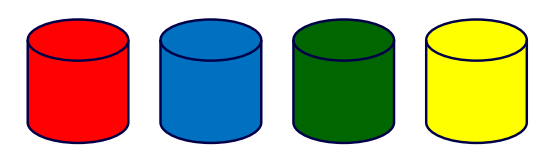
\includegraphics[width=\textwidth]{buildings.png}
\caption{Izgled zgradb}
\label{slika1}
\end{center}
\end{figure}


\pagebreak
\subsection{Zemljevid mesta}
\begin{figure}[!tbp]
  \centering
  \begin{minipage}[b]{0.2\textwidth}
	
\includegraphics[scale=0.6]{city.png}
	\caption{Skica mesta}
  \end{minipage}
  \hfill
  \begin{minipage}[b]{0.2\textwidth}
	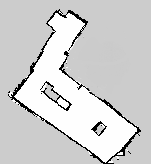
\includegraphics[scale=1]{robotMap.png}
	\caption{Mapa po kateri se je navigiral robot}
  \end{minipage}
\end{figure}



\section{\label{app-code}Programska koda}

TODO

\end{document}
